\section{A research agenda in AI for
science}\label{a-research-agenda-in-ai-for-science}

`AI for science' sits at a nexus of disciplines, methods, and
communities. Both AI and `science' (broadly defined) share a core
interest in learning from data. From this interest emerge different
research directions: for AI, questions about the nature of intelligence
and how to understand the learning process in humans and machines; for
science, the outputs of this learning process are the focus, with the
aim of adding new knowledge about natural, physical, and social systems.
A distinctive feature of the emerging `AI for science' agenda is the
ability to move between these worlds, using AI to drive progress in
science and taking inspiration from science to inspire progress in AI.
The result is a continuum of modelling approaches along a spectrum from
strongly mechanistic to statistical models, which allow researchers to
introduce or operate at different levels of abstraction.

The AI for science community therefore combines the ambitions of AI
research with domain-specific goals to advance the frontiers of research
and innovation in their discipline, with an engineering focus on
designing systems that work in deployment, while operating across scales
from the nano- to the interstellar. From these interfaces emerges a
research agenda that --- if successful --- promises to accelerate progress
across disciplines. Inspired by discussions at the Dagstuhl workshop, a
list of research questions arising from this agenda is given in Annex 2.
These span three themes:

\noindent\textbf{Building AI systems for science:} Attempts to deploy AI
in the context of scientific discovery have exposed a collection of gaps
in current machine learning and AI capabilities. Further work is needed
to develop the technical capabilities that will allow AI to be used more
effectively in research and innovation; developing those capabilities
also offers opportunities to contribute to wider attempts to deliver
sophisticated AI systems. Areas for progress include:

\begin{itemize}
\item
  Advancing methods, software and toolkits for high-quality simulation
  and emulation, which integrate effective uncertainty quantification
  and leverage advances in machine learning robustness to ensure the
  operate safely and effectively.
\item
  Detecting scientifically meaningful structure in data, through
  advances in causal machine learning.
\item
  Encoding domain knowledge in AI systems through integration of
  scientific laws, principles, symmetries, or invariances in machine
  learning models, and through virtual, autonomous systems to make
  research more effective.
\end{itemize}

\noindent\textbf{Combining human and machine intelligence:} Effective
deployment of AI in science requires effective interactions between
human, domain and machine intelligence across all stages of the
deployment pathway. AI systems can be made more effective by integrating
pre-existing knowledge about the system of study, but mechanisms are
needed to extract and encode that knowledge. Effective interfaces are
also required in the reverse direction. Translating the outputs of AI
analysis to increased human capability requires an understanding of what
insights are relevant, how they are best communicated, and the cultural
environment that shapes the conduct of science. Areas for progress
include:

\begin{itemize}
\item
  Designing interfaces between humans and machines or AI agents that can
  extract, formalise, and assimilate knowledge that domain researchers
  have acquired, including tacit knowledge, and that communicate new
  knowledge back to the user as actionable insights.
\item
  Building mechanisms for explainability that allow researchers to
  interrogate why and how an AI system delivered a particular result,
  with the explanations provided being tailored to user need.
\item
  Accelerating the pace of knowledge creation and use, through systems
  that mine the existing research knowledge base or that automate
  repetitive or time-consuming elements of the research process.
\end{itemize}

\noindent\textbf{Influencing practice and adoption:} By learning from
recent experiences of deploying AI for science, the field has an
opportunity to promote wider uptake and progress in both scientific
domains and in AI research. This requires capturing both the knowledge
that the community has already generated, about how to design AI
systems, and the know-how about how to overcome practical challenges
that accompanies it, while taking action to grow the community of
researchers excited about the potential of AI in science. Areas for
progress include:

\begin{itemize}
\item
  Supporting new applications, through challenge-led research programmes
  that promote interdisciplinary collaborations and support co-design of
  AI systems to help tackle scientific challenges.
\item
  Developing toolkits and user guides that allow researchers to
  understand which AI tools are suitable for which purposes, and how to
  deploy those tools in practice.
\item
  Sharing skills and know-how, through community outreach that
  disseminates knowledge and know-how in how to use AI.
\end{itemize}

Together, these areas for action highlight the importance of interfaces
-- between researchers and between modelling approaches -- in shaping
the development of AI for science (Figure 3).

\begin{figure}
\begin{center}
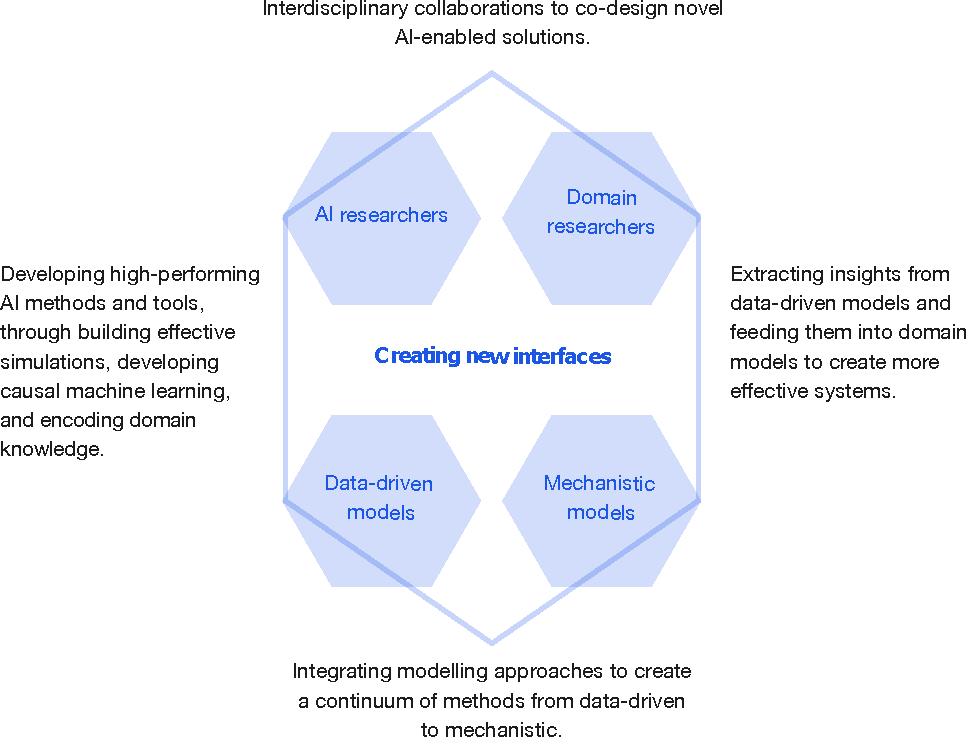
\includegraphics[width=\textwidth]{media/figure-3.pdf}
\caption{Interfaces between machine learning and domain researchers, and between data-driven and mechanistic models.}
\end{center}
\end{figure}
